\chapter{Methodology}


\section{Data set description}


MoleculeNet provides publicly available benchmark data sets for the prediction of 
various molecular properties.\cite{wu2018moleculenet} Here, the ESOL data set is used,
which contains the measured solubility at $25^{\circ} C$ in $log(mol/L)$ for $1110$ 
distinct small molecules, each represented as a SMILES string.\cite{delaney2004esol}
From this representation various chemical properties can be computed using the RDKit python package\cite{landrum2010r}. 
The following properties are used to create the node feature vector: \cite{wu2023chemistry}

\begin{itemize}
    \item \textbf{Atom symbol:} One hot encoding of the atom type \\
        $\left( [B, C, N, O, F, Si, P, S, Cl, As, Se, Br, Te, I, At, metal] \right)$
    \item \textbf{Degree:} Number of covalent bonds (minimum is $0$ and maximum is $5$)
    \item \textbf{Formal charge:}\cite{parkin2006valence} The formal charge of an atom is defined as the difference between its valence 
        electrons and the number of electrons assigned from the Lewis structure where each single bond 
        contributes one electron. For example, nitrogen $(N)$ in nitrobenzene (\cref{fig:nitrobenzene})
        has a formal charge of $+1$, because $N$ has five valence electrons and gets four electrons 
        from the Lewis structure (one electron from each of the single bonds and two from the double bond).

        \begin{figure}[h]
            \centering
            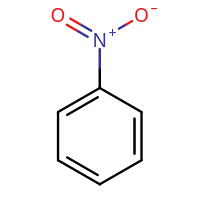
\includegraphics[scale=0.5]{nitrobenzene.png}
            \caption{Lewis structure of nitrobenzene}
            \label{fig:nitrobenzene}
        \end{figure}

    \item \textbf{Hybridization:}\cite{alabugin2015orbital} One hot encoding of the orbital structure of the atom \\
        $\left([sp, sp^2, sp^3, sp^3d, sp^3d^2, other]\right)$)

    \item \textbf{Aromaticity:} An aromatic system is a ring containing a delocalized electron 
        structure with $4n + 2$ electrons. For example, the benzene ring in \cref{fig:nitrobenzene}
        is an aromatic structure. ($0$ or $1$)

    \item \textbf{Hydrogens:} Hydrogen atoms are treated implicitly in order to prevent the
        explosion of the number of nodes in a molecular graph. If hydrogen atoms 
        were treated explicitly, then nitrobenzene (\cref{fig:nitrobenzene}) would 
        already have five more nodes, increasing the total nodes from ten to fifteen.
        (One hot encoding: $[0, 1, 2, 3, 4]$)

    \item \textbf{Chirality:}\cite{prelog1976chirality} Indicates whether the atom is a chiral center. Chirality 
        occurs when for example a carbon atom is bonded to four different groups. 
        Then the spatial orientation of those groups matters as not all configurations 
        are equivalent under rotation. ($0$ or $1$)

    \item \textbf{Chirality type:} One hot encoding of the chirality type $([R, S])$.

\end{itemize}


The type of an edge is determined by a bond feature vector consisting of the following chemical properties:


\begin{itemize}
    \item \textbf{Bond type:} One hot encoding of bond type ([single, double, triple, aromatic])
    \item \textbf{Conjugation:} Indicates whether the bond is part of a delocalized electron strucure.
        ($0$ or $1$) 
    \item \textbf{Ring:} Indicates whether the bond is part of a ring ($0$ or $1$).
    \item \textbf{Stereo:} One hot encoding of stereo configuration of the bond.
        ([StereoNone, StereoAny, StereoZ, StereoE])
\end{itemize}


\section{Architecture of the graph neural network model to predict water solubility}


Prediction of water solubility is achieved using the same RGCN model as Wu et. al. (\cref{fig:ml_model}),
with the hyper parameters listed in \cref{tab:hyperparameters}. To obtain more 
robust predictions, ten models are trained, each with a different seed 
$(2023 + 10i, \text{ with } i \in \{1, 2, \dots, 10\})$, where the final 
prediction is then obtained by the average prediction over all models.\cite{wu2023chemistry} 
The model is implemented in python using PyTorch Geometric\cite{Fey/Lenssen/2019}, training progress 
is tracked using wandb\cite{wandb} and analysis of the results is done using 
pandas\cite{reback2020pandas} an plotly\cite{plotly}.


\begin{figure}[h]
    \centering
    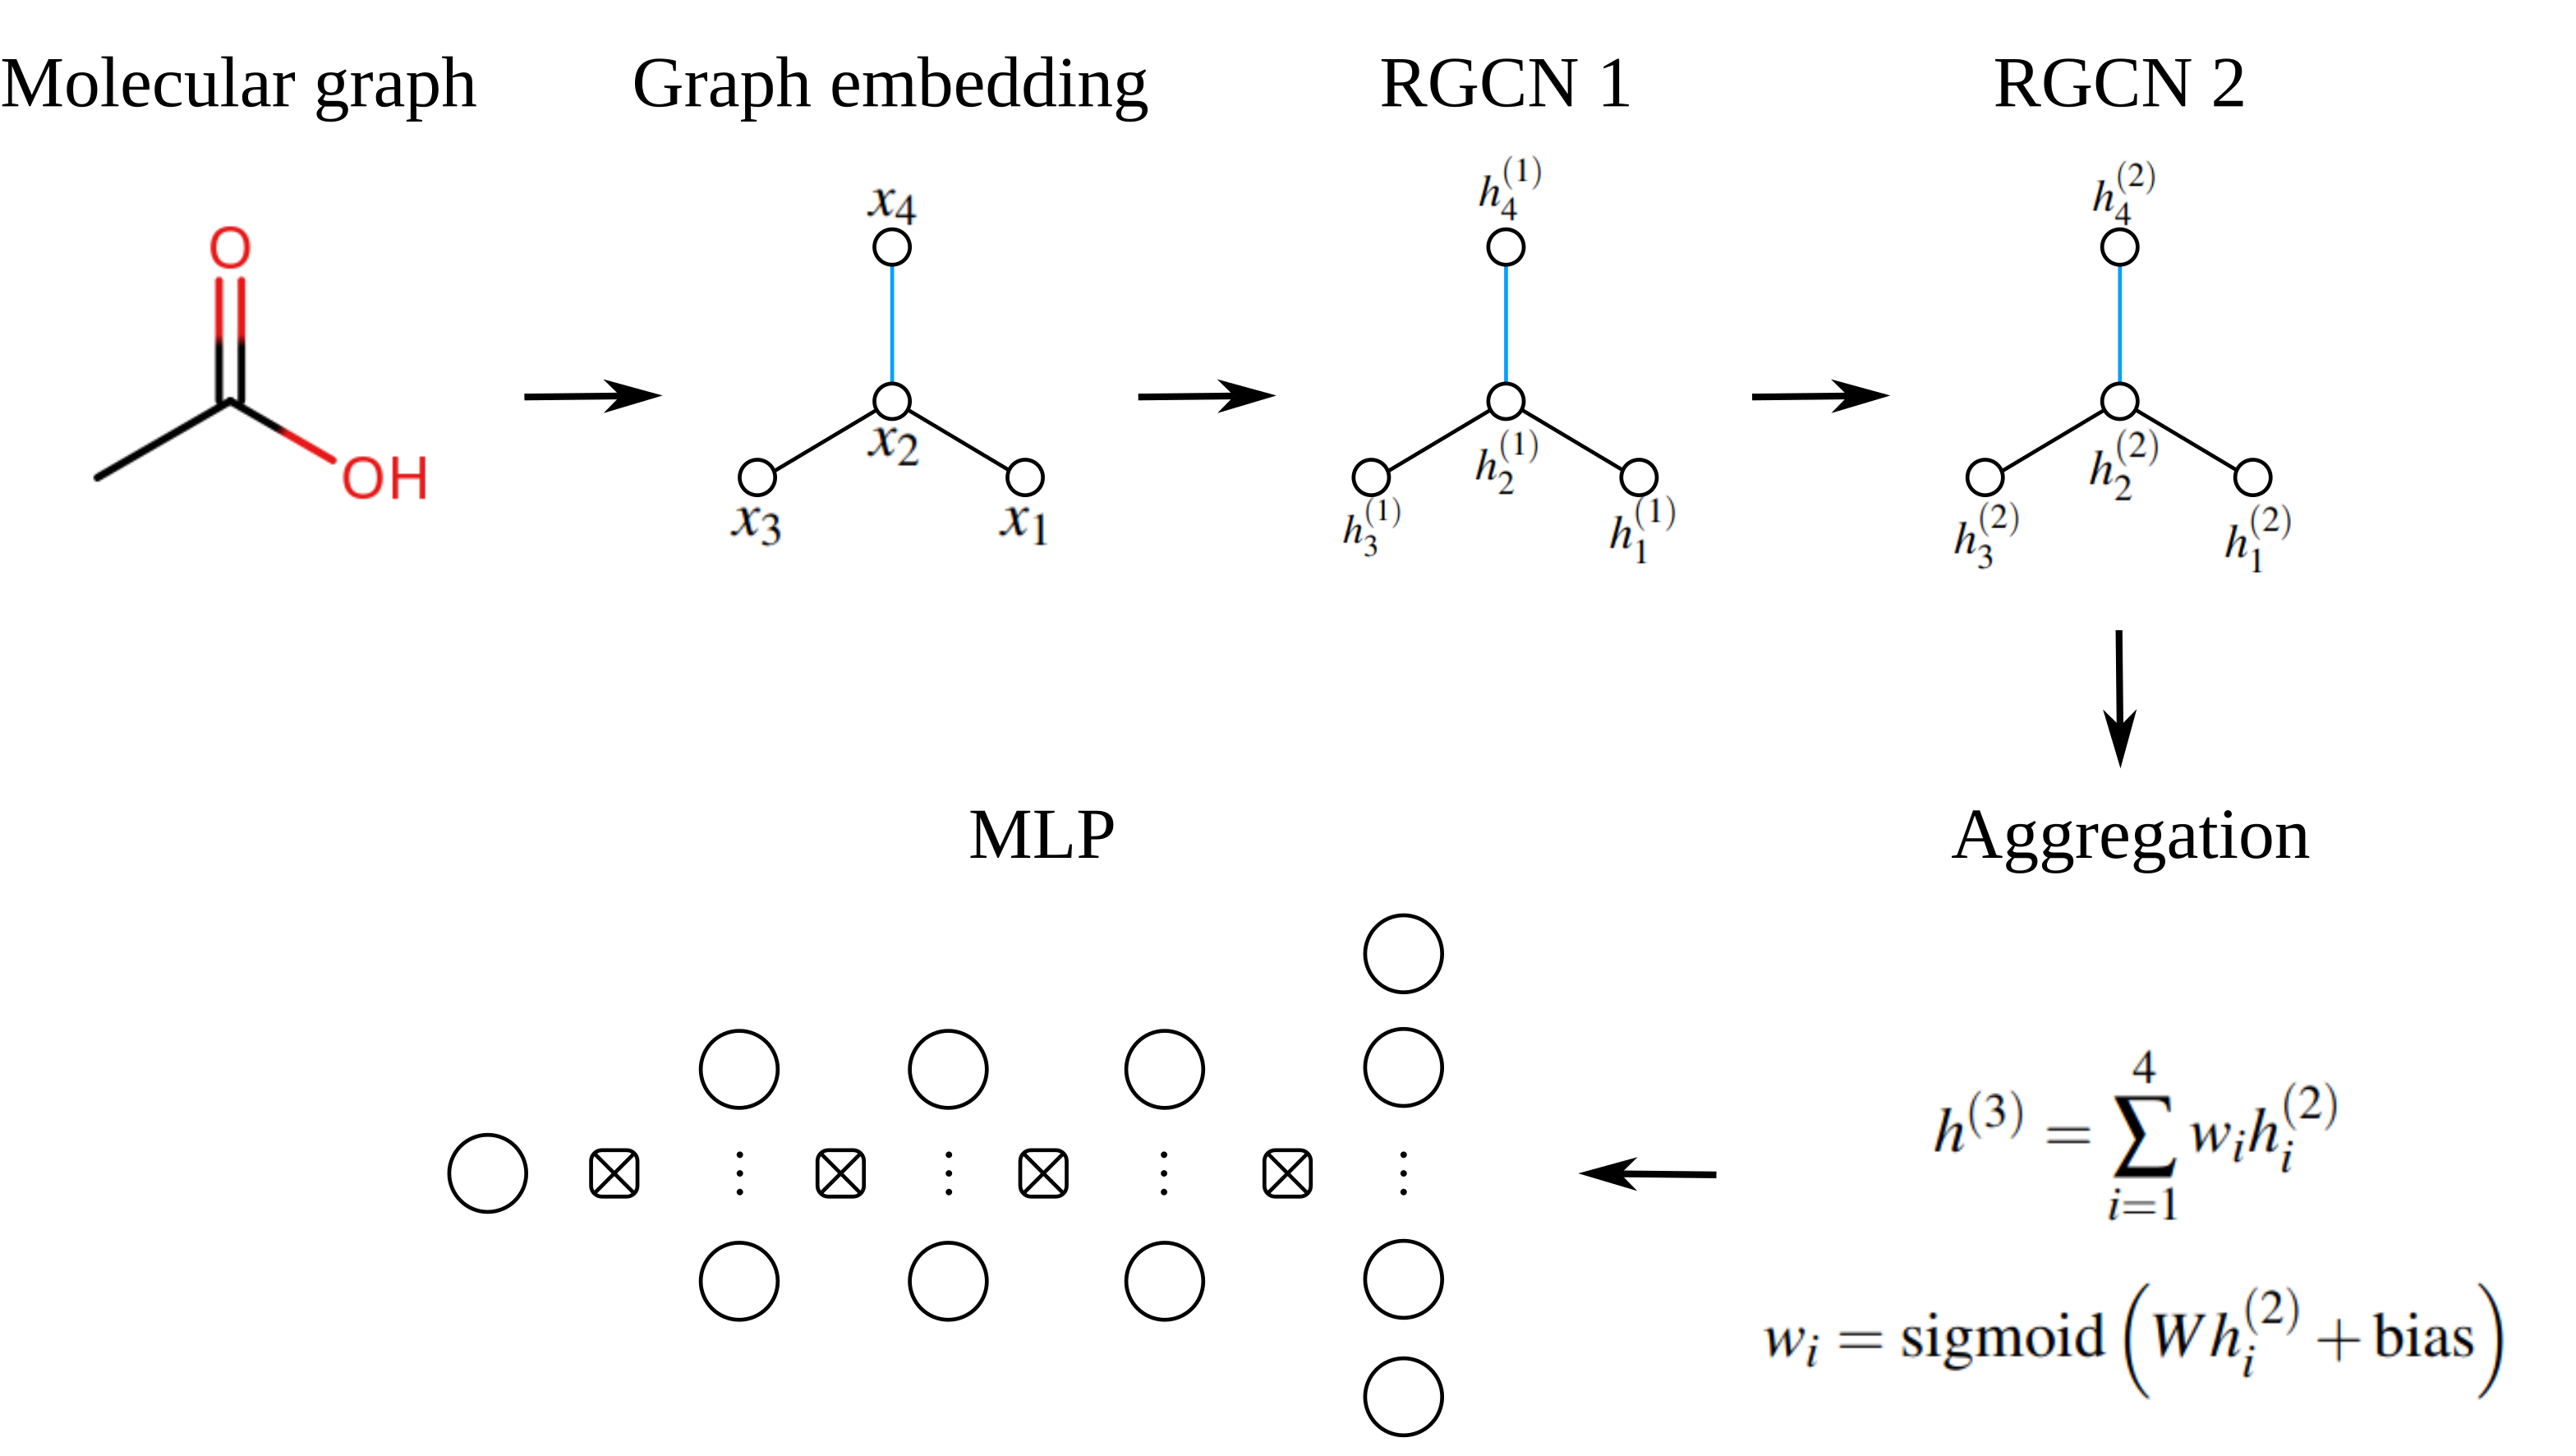
\includegraphics[scale=0.85]{rgcn_model.png}
    \caption{Machine learning model used for the prediction of water solubility of 
        small molecules. First, the molecular graph is embedded to a graph where the 
        bond features are used to determine edge types and node features are computed 
        using the RDKit python package. Next, two RGCN layers are applied, which are 
        followed by a weighted sum to aggregate the whole graph into one vector. This 
        vector is then passed to an MLP to obtain the final prediction.
    }
    \label{fig:ml_model}
\end{figure}


\begin{table}[h]
    \caption{ Hyper parameters from \protect\citen{wu2023chemistry} of an RGCN model to predict water solubility.}
    \label{tab:hyperparameters}
    \begin{center}
        \begin{tabular}{cc}
            \toprule
            \textbf{hyper parameter} & \textbf{value} \\
            \midrule
            RGCN layers & 2 \\
            RGCN hidden units & 256 \\
            RGCN dropout rate (each layer) & 0.5 \\
            MLP hidden units & 64 \\
            MLP dropout rate (each layer) & 0.1 \\ 
            Epochs & 500 \\
            Early stop & 30 \\
            \bottomrule
        \end{tabular}
    \end{center}
\end{table}


\newpage

\section{Chemical expectations}


Because water is a polar molecule, substructures that increase the overall polarity 
of a molecule, will also increase the water solubility and hence are expected to obtain 
a positive attribution. Furthermore, when a substructure has the ability to form hydrogen 
bonds, it should have a higher positive attribution than when no hydrogen bonds can be 
formed. On the other hand, apolar substructures such as large carbon chains and polycyclic
compounds reduce the effect of smaller polar groups, resulting in a reduced 
water solubility. Therefore, apolar substructures should have negative attributions. 


\section{Substructures}


To subdivide a molecule into its functional groups and main structure (referred to as scaffold),
a list of commonly occurring functional groups in small molecules is created together with their 
respective SMILES arbitrary target specification (SMARTS)\cite{smartsDaylight} to allow pattern 
matching using RDKit (\cref{app:functional_groups_list}). Some molecules do not 
have any of the specified functional groups or can 
be more intuitively partitioned using breaking retrosynthetically interesting chemical substructures 
(BRICS)\cite{degen2008art}. BRICS splits a molecule into substructures that could possibly used 
in a chemical reaction that synthesizes the original molecule. 


When ranking the molecules to compute the Spearman correlation coefficient, it is more 
meaningful when more than two substructures are present; otherwise, the outcome is binary.
Therefore, when Spearman rank correlation is used, it can be assumed that the substructure 
method (functional groups or BRICS) that yields the most substructures is chosen to partition
the molecule.


